% -*- root: ../thesis.tex -*-
%!TEX root = ../thesis.tex
% ******************************* Thesis Chapter 7 ****************************

% ----------------------- paths to graphics ------------------------

% change according to folder and file names
\graphicspath{{8/figures/}}
% ----------------------- contents from here ------------------------
This chapter presents both discussions and extensions on the models and ideas presented in Chapters~\ref{ch:classification},~\ref{ch:multi-class},~\ref{ch:general}.
All figures presented are reproducible by running the examples provided in the GitHub repository \url{https://github.com/theogf/Phd-Thesis}.
Section~\ref{sec:further} considers how augmentations can be generalized further and what analysis we need to fully understand the improvement brought by augmentations.
Section~\ref{sec:heteroscedastic} presents new augmented models for \ac{GP} regression with heteroscedastic noise.
Section~\ref{sec:hmc_vs_gibbs} explores how \ac{HMC} could be used (or not) with augmented models.
Section~\ref{sec:improvemulticlass} shows how the multi-class model of Chapter~\ref{ch:multi-class} can be improved in multiple ways.
Section~\ref{sec:sample_sparse} presents a way to combine inducing points and sampling using augmentations.
Finally, Section~\ref{sec:limits} consider more largely the limitations existing with our augmentation approach.

\section{Further generalizations and understanding}
\label{sec:further}
The works presented in this thesis only scratched the surface of how helpful mixtures and representations are.
\paragraph{Moment Generating Functions}\mbox{}\\
We are still exploring ways to identify larger classes of functions identifiable as scale mixtures or hierarchical mixtures.
Already mentioned in Chapters~\ref{ch:multi-class} and \ref{ch:general},
the connection with the \acf{MGF} of a distribution is a promising direction.
We already identified augmentable functions as being a transformed \ac{MGF} of the augmented variables in Chapter~\ref{ch:general}:
\begin{align*}
    \varphi(x^2) = \int_0^\infty e^{-x^2\omega}p(\omega)d\omega \forall x \in \mathbb{R} \;\equiv\; \mathrm{MGF}_{p(\omega)}(x) = \varphi(-\sqrt{x}),\qquad \forall x \geq 0.
\end{align*}
However, this is limited to \ac{MGF} of continuous variables with a square transformation on the inputs.
We can extend the notion of augmentable functions to \ac{MGF} of discrete and multivariate distributions, where the domain of $\omega$ is not always $\mathbb{R}^+$.
For example, we used the \ac{MGF} of a Poisson distribution in Chapter~\ref{ch:multi-class}:
\begin{align*}
    \exp(\lambda(e^x - 1)) = \sum_{n=0}^\infty e^{n e^x} \Po(n|\lambda).
\end{align*}
It is not a scale mixture of Gaussians, but with the right variable transformations, it can still be useful.
The \ac{MGF} of a Poisson is known, but we could also consider arbitrary \ac{MGF} since we are able to sample from a distribution given its Laplace transform only \cite{ridout2009generating}.

The \ac{MGF} is also an interesting tool for creating hierarchical models. 
Since the \ac{MGF} is of the form $\sum_{x} e^{tx} p(x)$ or $\int e^{tx}p(x)dx$, by setting $t=\log \sigma(f)$, we get scales mixtures of the form $\sum_x \sigma^x(f)$.
Thanks to the property that $\sigma^n(f)$ is augmentable for any $n\in \mathbb{R}^+$, we can use P\'olya-Gamma variables and obtain a conditionally conjugate model for a \ac{GP}.
Additional examples of such constructions are shown in this chapter in Sections \ref{sec:heteroscedastic} and \ref{sec:improvemulticlass}.

\paragraph{Marginalizing out augmented variables}\mbox{}\\
A potential improvement for augmented models is the identification of marginalizable augmented variables that keep the conditional conjugacy of the model.
For example, in the multi-class model from Chapter~\ref{ch:multi-class}, the augmented variable $\lambda$ can be marginalized out, as shown in Section~\ref{sec:improvemulticlass}.
We can reduce the dimensionality of the model and avoid tricky situations like the inner loop updates in Chapter~\ref{ch:multi-class}.
This marginalization step is avoidable by identifying the right \ac{MGF} from the start.
As shown in Section~\ref{sec:heteroscedastic_nongaussian}, switching between marginalized and augmented models gives great inference flexibility.

\paragraph{Convergence speed analysis}\mbox{}\\
An unfinished work (despite trying) is to establish convergence rates (error as a function of the number of iterations) for the \ac{CAVI} algorithm and derive theoretical bounds on the intra-chain correlation and of the ergodicity for the Gibbs sampler.
Experimental results indicate that the error on the variational free energy (and variational parameters) is decreasing as $\|\VFE^{*} - \VFE^{t}\|\propto C_0 e^{-ct}$, where $t$ is the number of iterations, but we did not manage to write a formal proof.
We show the decay for both the variational free energy and the variational parameters for different examples in Figure~\ref{fig:convergence}.

\begin{figure}[H]
\centering
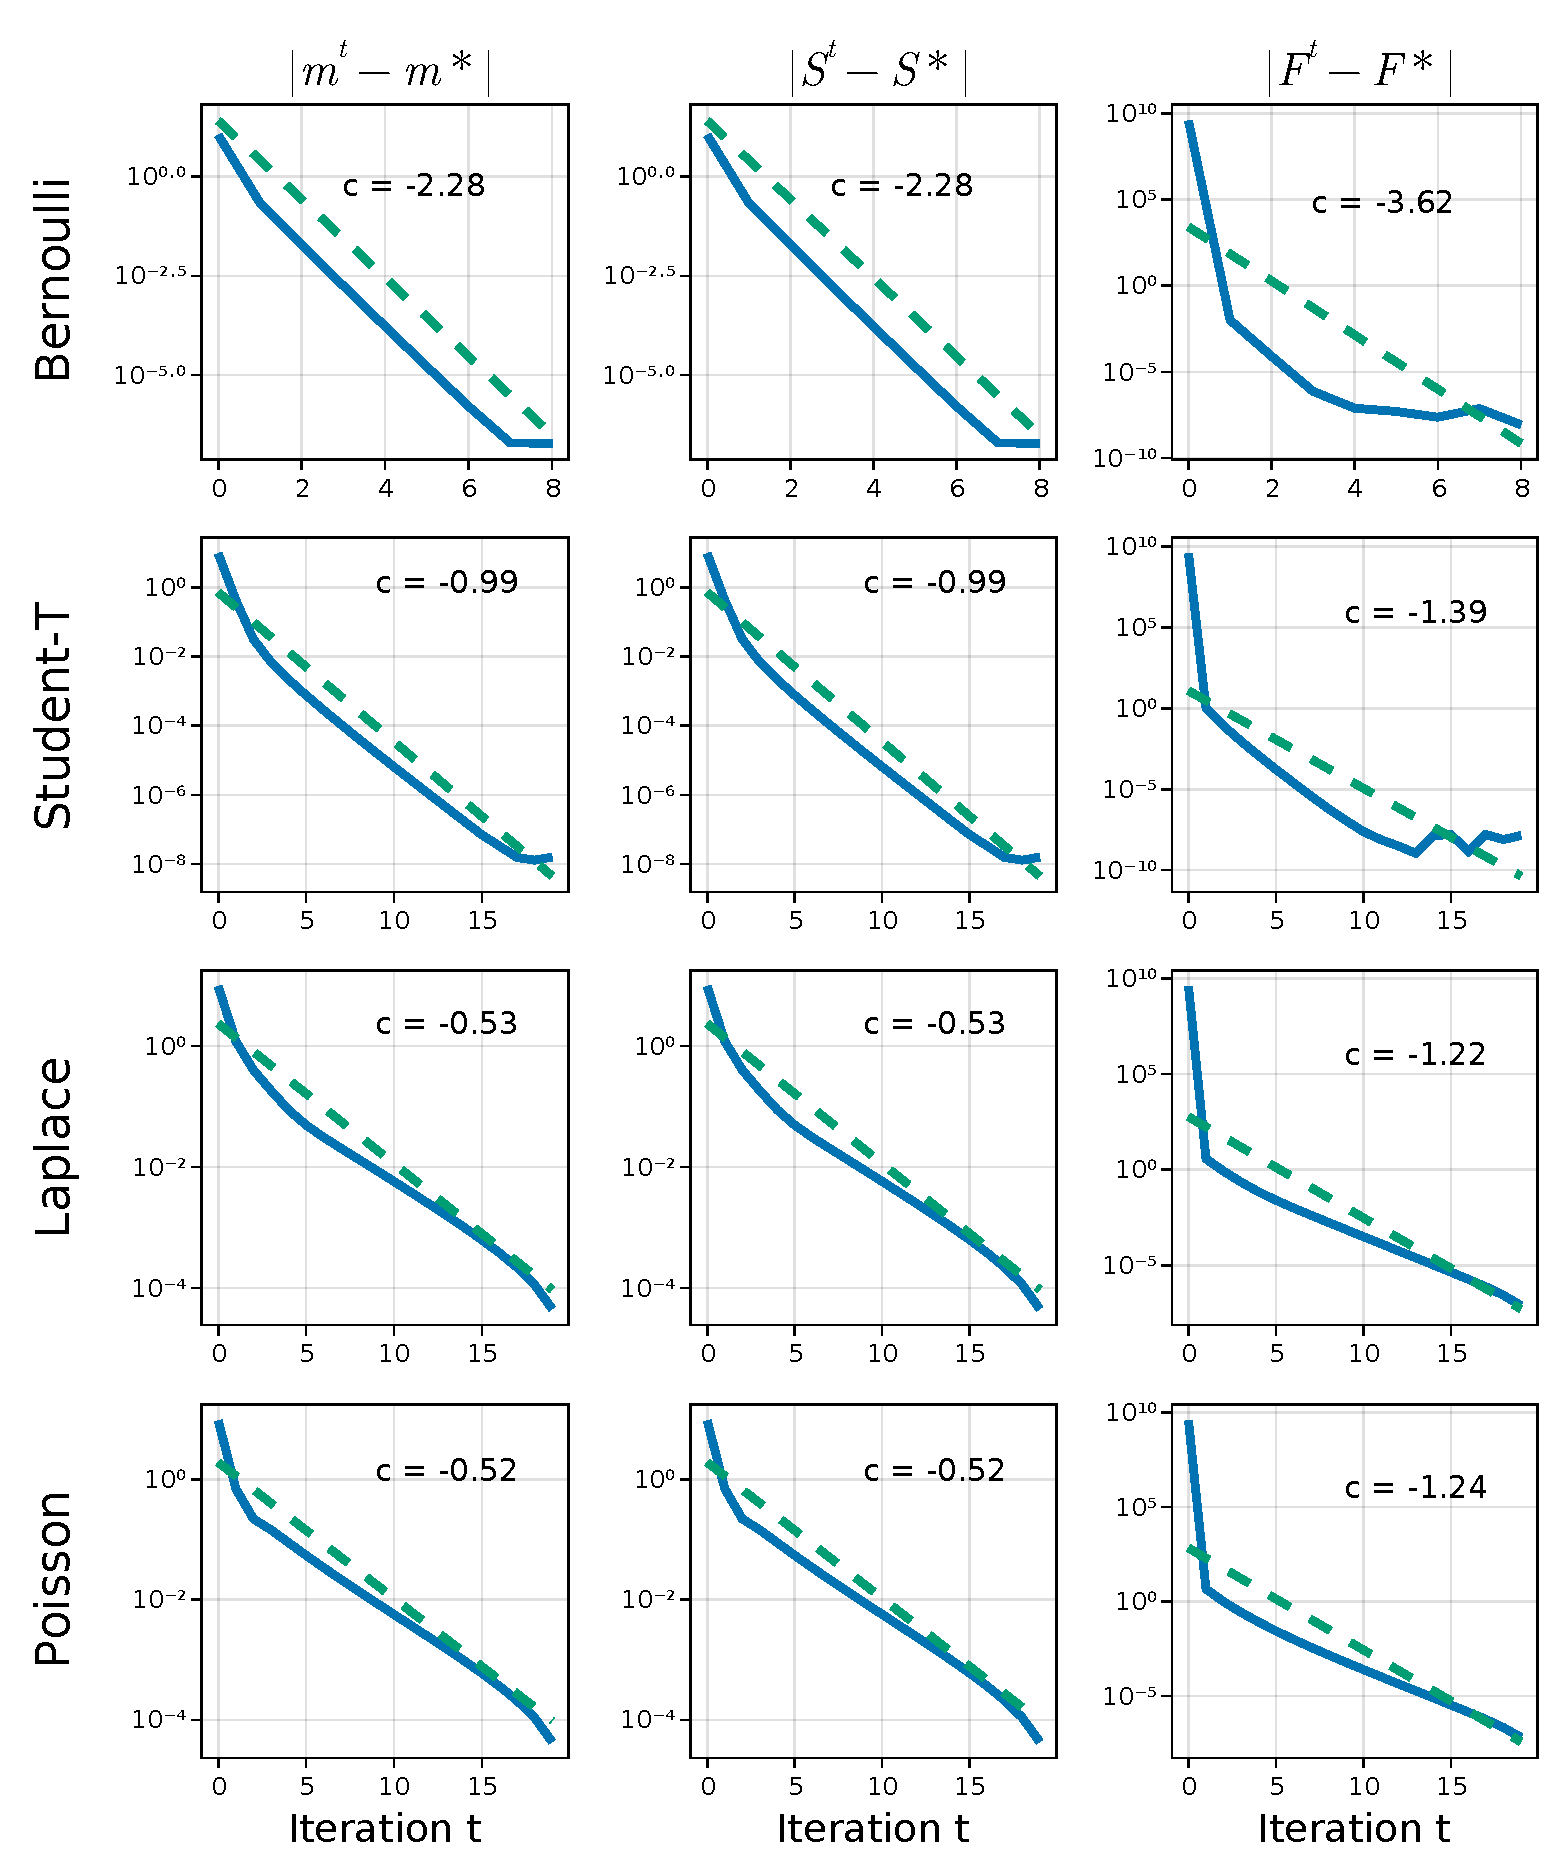
\includegraphics[width=\textwidth]{./chapters/8_discussions/figures/convergence.pdf}
\caption{Convergence plot of the \ac{CAVI} updates for a one-dimensional toy example with different likelihoods (y-axis in log scale).
The solid blue line shows the empirical error over the number of iterations and the dashed green line shows the fit of the function $C_0 \exp(c t)$.
The exponential coefficient is written down explicitly for each likelihood.}
\label{fig:convergence}
\end{figure}


\section{Double bounds for intricate latent \acsp{GP}}
\label{sec:heteroscedastic}
The multi-class model developed in Chapter~\ref{ch:multi-class} paves the way to work with multi-latent models and hierarchical augmentations.
Based on this idea, we developed another multi-latent model on the heteroscedastic regression likelihood  \cite{wangGaussianProcessRegression2012,lazaro2011variational}.
It models simultaneously the mean and variance of a regression likelihood with two latent \acp{GP} $f$ and $g$.
We consider both Gaussian and Non-Gaussian likelihoods since we can stack augmentations.
We start with the simplest model: the heteroscedastic Gaussian likelihood.

\subsection{Heteroscedastic Gaussian Likelihood}
\label{sec:hetero_gaussian}
A crucial model choice is the function mapping $g$ to the likelihood variance $\epsilon^2$.
The exponential link, i.e. $\epsilon^2(x) = \exp(g(x))$, is the most popular, however to be able to apply our augmentations, we use the link $\epsilon^2(x) = \left(\lambda \sigma(g(x))\right)^{-1}$.
Let's look at the case of the heteroscedastic Gaussian likelihood, defined as:
\begin{align}
    p(y|f,g,\lambda) = \frac{\sqrt{\lambda \sigma(g)}}{\sqrt{2\pi}}\exp\left(-\frac{\lambda \sigma(g)(y-f)^2}{2}\right).\label{eq:hetero_lik}
\end{align}

The augmentations for this likelihood are straightforward and quite similar to the multi-class ones from Chapter~\ref{ch:multi-class}.
\begin{align}
    \exp\left(-\frac{\lambda\sigma(g)(y-f)^2}{2}\right) =& \exp\left(\frac{\lambda(\sigma(-g) -1)(y-f)^2}{2}\right)\nonumber\\
    =&\sum_{n=0}^\infty \sigma^n(-g)\Po \left(n~\middle|~\frac{\lambda(y-f)^2}{2}\right),\label{eq:aug_poisson}
\end{align}
where we used the \ac{MGF} of the Poisson distribution.
Using the P\'olya-Gamma augmentation and the additivity property of P\'olya-Gamma variables, we get the final augmented likelihood:
\begin{align}
    p(y,n,\omega\mid f,g,\lambda) = \frac{\sqrt{\lambda}}{2^n\sqrt{\pi}}\exp\left(\frac{1}{2}\left(g\left(\frac{1}{2}-n\right) - \frac{g^2}{\omega}\right)\right)\PG \left(\omega \mid \half + n, 0\right) \Po \left(n \mid \lambda\frac{(y-f)^2}{2}\right)\label{eq:heteroscedastic}
\end{align}
The interesting part about this augmented likelihood~\eqref{eq:heteroscedastic} is that although it is conditionally conjugate in $g$, $\omega$, and $n$, it is unclear how to infer $f$:
it is quadratic in $g$ but not in $f$.
It turns out that the Gibbs sampler for this model is very simple:
We take the augmented likelihood $p(y,\omega,n|f,g,\lambda)$, marginalize out $n$ and $\omega$ and, as expected, we get the original likelihood~\eqref{eq:hetero_lik}, which is conditionally conjugate with $f$.
The conditional $p(f|y,g,\lambda)$ on this likelihood is the \textbf{collapsed conditional}.
In a Gibbs sampling scheme, this allows us to perform a \textbf{collapsed step}.
We give all the Gibbs sampling steps in Algorithm~\ref{alg:gibbs_hetero}.
So far, we have excluded the $\lambda$ parameter from inference.
By putting a Gamma prior $\Ga(\lambda|\alpha, \beta)$, where $\alpha$ is the shape and $\beta$ is the rate, the collapsed conditional is available in closed-form:
\begin{align*}
    p(\lambda|\boldf, \boldg, \boldy) = \Ga(\lambda| \alpha + \frac{N}{2}, \beta + \sum_{i=1}^N \frac{\sigma(g^i)}{2}(y^i - f^i)^2).
\end{align*}


As underlined in Section~\ref{sec:cavi}, the \ac{CAVI} updates need the model's full conditionals and are not compatible with collapsed conditionals.
To solve this problem, we need to reverse-engineer how \ac{CAVI} updates are obtained and start with a first bound on the \ac{KL} divergence:
\begin{align*}
    \KL{q(\boldf)q(\boldg)}{p(\boldf,\boldg|\boldy)}\leq& \min_{q(\boldg)}-\expec{q(\boldg)}{\expec{q(\boldf)}{\log p(\boldy|\boldf,\boldg)}} + \KL{q(\boldf)q(\boldg)}{p(\boldf)p(\boldg)} - \log p(\boldy)\\
    =& \min_{q(\boldg)}-\expec{q(\boldg)}{\log p(\boldy|\boldg, \bmu^*_f,\bSigma^*_f)} + \KL{q(\boldg)}{p(\boldg)} + \operatorname{KL}_f^* - \log p(\boldy)= \mathcal{F}_1.
\end{align*}
$p(\boldy|\boldg, \bmu^*_f, \bSigma^*_f)$ and $\mathrm{KL}^*_f$ are expectations computed with the optimal $q^*(\boldf)=\mathcal{N}\left(\boldf|\bmu_f^*,\bSigma_f^*\right)$.
We can now use the augmentations from Equation~\eqref{eq:heteroscedastic} on the expected log-likelihood, where we replaced $(y_i-f_i)^2$ by $(y_i - (\bmu_f^*)_i)^2 + (\Sigma_f^*)_{ii}$, and build a second bound.

\begin{align}
    \mathcal{F}_1 \leq \min_{q(\boldg)q(\bomega,\bn)} \expec{q(\boldg)q(\bomega,\bn)}{\log p(\bomega,\bn,\boldy|\boldg,\bmu_f^*,\bSigma_f^*)} + \KL{q(\boldg)}{p(\boldg)} + \operatorname{KL}_f^*=\mathcal{F}_2 \label{eq:second_bound}
\end{align}

It is straightforward to find the optimal variational distributions $q^*(\boldg)$ and $q^*(\bomega,\bn)$ minimizing $\mathcal{F}_2$ which allows us to use \ac{CAVI} updates.
Then, injecting the optimal distribution $q^*(\boldg)q(\bomega,\bn)$ in $\mathcal{F}_2$, we can derive the optimal $\bmu_f^*$ and $\bSigma_f^*$, obtainable in closed-form.
The resulting \ac{CAVI} updates are given in Algorithm~\ref{alg:cavi_hetero}.
For $\lambda$, we can use the second bound \eqref{eq:second_bound} and obtain a closed-form maximum-likelihood estimate, given in Algorithm~\ref{alg:cavi_hetero}.

This double-bound approach is very similar to \citet{lazaro2011variational}, although they are using the exponential link and need some extra computations.

\begin{algorithm}[H]
    \caption{Gibbs sampling for the Heteroscedastic Gaussian likelihood}
    \begin{algorithmic}
        \State \textbf{input:} $\boldf,\boldg, \lambda, \boldy$, $p(\boldf,\boldg) = \mathcal{N}(\boldf|\bmu^0_f, K)\mathcal{N}(\boldg|\bmu^0_g, K)$, $p(\lambda|\alpha,\beta)$.
        \For{$t$ in $1:$ N samples}
            \State Draw $\lambda \sim p(\lambda|\boldf,\boldg,\boldy) = \Ga(\lambda| \alpha + \frac{N}{2}, \beta + \sum_{i=1}^N \frac{\sigma(g^i)}{2}(y^i - f^i)^2).$
            \State Draw $n^i \sim p(n^i|f^i, g^i, \lambda) = \Po(\lambda \sigma(-g^i) \frac{(y^i - f^i)^2}{2})$
            \State Draw $\omega^i \sim p(\omega^i|n^i,g^i) = \PG(0.5 + n^i, |g^i)$
            \State Draw $\boldg \sim p(\boldg|\boldn, \bomega) = \mathcal{N}(\bmu_g,\bSigma_g)$
            \State \quad where $\bSigma_g=  \left(K^{-1} + \diag(\bomega)\right)^{-1}$ and $\bmu_g = \bSigma_g\left(K^{-1}\bmu^0_g + \frac{0.5 - \boldn}{2}\right)$
            \State Draw $\boldf \sim p(\boldf | \boldg, \lambda) = \mathcal{N}(\bmu_f,\bSigma_f)$
            \State \quad where $\bSigma_f = \left(K^{-1} + \lambda\diag(\sigma(\boldg))\right)^{-1}$ and $\bmu_f = \bSigma_f\left(K^{-1}\bmu_f^0 + \lambda\diag(\sigma(\boldg))\frac{\boldy}{2}\right)$
        \EndFor
    \end{algorithmic}
    \label{alg:gibbs_hetero}
\end{algorithm}

\begin{algorithm}[H]
    \caption{\ac{CAVI} Updates for the Heteroscedastic Gaussian likelihood}
    \begin{algorithmic}
        \State \textbf{input:} $q(\boldf,\boldg) = \mathcal{N}(\boldf|\bmu_f,\bSigma_f)\mathcal{N}(\boldg|\bmu_g,\bSigma_g)$, $p(\boldf,\boldg) = \mathcal{N}(\boldf|\bmu^0_f, K)\mathcal{N}(\boldg|\bmu^0_g, K)$, $\boldy$ and $\lambda$.
        \While{convergence criteria is not met}
            \State $\psi^i = \widetilde{\sigma}(q(g^i))$
            \State $\lambda = \frac{N}{\sum_{i=1}^N (1 - \psi^i)\sqrt{(y^i - \mu_f^i)^2 + \Sigma_f^{ii}}}$
            \State $\gamma^i = \frac{\lambda}{2} \psi^i  \sqrt{(y^i - \mu_f^i)^2 + \Sigma_f^{ii}}$
            \State $c^i = \sqrt{(\mu_g^i)^2 + \Sigma^{ii}_g}$
            \State $\theta^i = \expec{q(\omega^i|n^i)q(n^i)}{\omega^i} = \frac{0.5 + \gamma^i}{2c^i}\tanh\left(\frac{c^i}{2}\right)$
            \State $\bSigma_f = \left(K^{-1} + \lambda\diag(1-\boldsymbol{\psi})\right)^{-1}$
            \State $\bmu_f = \bSigma_f\left(K^{-1}\bmu_f^0 + \lambda\diag(1 - \boldsymbol{\psi}) \boldy\right)$
            \State $\bSigma_g = \left(K^{-1} + \diag(\btheta)\right)^{-1}$
            \State $\bmu_g = \bSigma_g\left(K^{-1}\bmu_g^0 + \frac{0.5 + \bgamma}{2}\right)$
        \EndWhile
    \end{algorithmic}
    where $q(\boldn, \bomega) = \prod_{i=1}^N \PG(\omega^i|0.5 + n, c^i)\Po(n^i|\gamma^i)$ and $\widetilde{\sigma}(q(g^i)) = \frac{e^{-\mu_g^i/2}}{\sqrt{(\mu_g^i)^2 + \Sigma^{ii}_k} / 2}$ can be seen as a close approximation to $\expec{q(g^i)}{\sigma(-g^i)}$.
    \label{alg:cavi_hetero}
\end{algorithm}

A 1-dimensional toy example is shown in Figure~\ref{fig:heteroscedastic} with the results of the inference algorithms.

\begin{figure}[H]
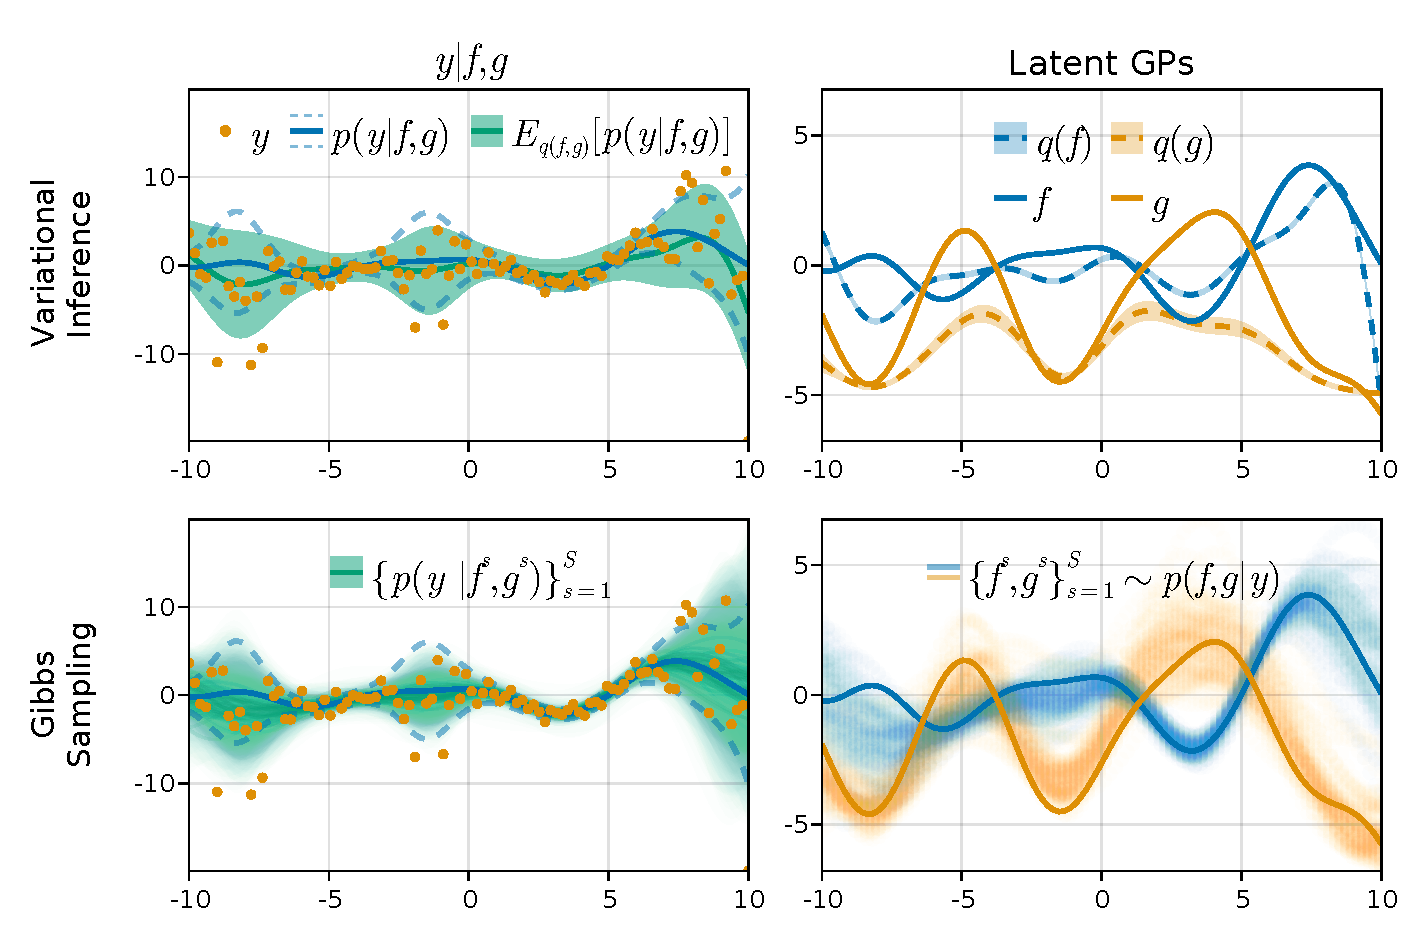
\includegraphics[width=\textwidth]{./chapters/8_discussions/figures/heteroscedastic.pdf}
\caption{Toy example of a heteroscedastic Gaussian regression problem and the resulting inference from Algorithm ~\ref{alg:gibbs_hetero} (Gibbs sampling, bottom plots) and Algorithm~\ref{alg:cavi_hetero} (Variational Inference, top plots).
The left plots show the output space.
The training data $\boldy$ are in orange, the generating likelihood is shown in blue (mean in solid line and one standard deviation in dashed-line).
The green bands show the predictive distributions with one standard deviation obtained after posterior inference (one band for variational inference and cumulative bands for the sampling approach).
The right plots show the true latent functions $f$ and $g$ used to generate $y$ as well as the inferred posteriors: variational on top (mean with one standard deviation) and samples at the bottom.}
\label{fig:heteroscedastic}
\end{figure}

We can see that on this one-dimensional example, \ac{VI} but more particularly Gibbs sampling, manage to recover the original model.
For \ac{VI}, the variance on the latent $f$ is almost negligible since all the data variance is absorbed into the likelihood variance term.
The samples obtained with Gibbs sampling, without any warmup, fit nicely the true processes of $f$ and $g$.

An implementation as well as detailed derivations are in the \href{https://github.com/JuliaGaussianProcesses/AugmentedGPLikelihoods.jl}{AugmentedGPLikelihoods.jl} package \cite{theo_galy_fajou_2022_6347022}.

\subsection{Heteroscedastic Non-Gaussian Likelihood}
\label{sec:heteroscedastic_nongaussian}
This method extends to non-Gaussian likelihoods as well.
We take the example of the heteroscedastic Student-t likelihood, where we have a local scale with standard deviation $\epsilon(x) = \lambda \sigma(g)$ with $\lambda \in \mathbb{R}^+$.

Similar to the heteroscedastic Gaussian likelihood~\eqref{eq:hetero_lik}, we get the likelihood:
\begin{align}
    p(y|f,g,\lambda,\nu) = \frac{\Gamma(\frac{\nu+1}{2})\sqrt{\lambda\sigma(g)}}{\Gamma(\frac{\nu}{2})\sqrt{\pi\nu}}\left(1 + \lambda \sigma(g)\frac{(y-f)^2}{\nu}\right)^{-\frac{\nu+1}{2}}
    \label{eq:hetero_studentt}
\end{align}

To simplify the notation, we define the scaled residuals $\Delta=\Delta_\nu(f,y,\lambda) = \frac{\lambda(y-f)^2}{\nu}$, $\alpha =\frac{\nu+1}{2}$ and the normalization constant $Z = \frac{\Gamma(\frac{\nu+1}{2})}{\Gamma(\frac{\nu}{2})}$.
We can proceed with the first augmentation:
\begin{align}
    (1 + \sigma(g)\Delta)^{-\alpha} =& (1 + \Delta(1 - \sigma(-g)))^{-\alpha}\nonumber\\
    =&(1 + \Delta - \Delta\sigma(-g))^{-\alpha}\nonumber\\
    =& (\Delta\sigma(-g))^{-\alpha}\left(\frac{\sigma(-g)\Delta}{1 + \Delta -\sigma(-g)\Delta}\right)\nonumber\\
    =&\sum_{k=0}^{\infty} \Delta^k \mathrm{NB}(k|\sigma(-g),\alpha),\label{eq:negativebinomial}
\end{align}
where we used the \ac{MGF} of the \textbf{Negative Binomial} distribution.

We obtain the same result by performing first the augmentation of the Student-t with a Gamma variable:
\begin{align}
    p(y|f,g,\lambda) =& \int_0^\infty \mathcal{N}(y| f, (\lambda\sigma(g)\gamma)^{-1})\mathrm{IG}(\gamma|\frac{\nu}{2},\frac{\nu}{2})d\gamma\nonumber\\
    p(y,\gamma|f,g,\lambda)=& \mathcal{N}(y| f, (\lambda\sigma(g)\gamma)^{-1})\mathrm{IG}\left(\gamma|\frac{\nu}{2},\frac{\nu}{2}\right).\label{eq:aug_gamma_studentt}
\end{align}
$\mathcal{N}(y| f, (\lambda\sigma(g)\gamma)^{-1})$ is the same starting point as Equation~\eqref{eq:hetero_lik} with an additional scaling $\gamma$.
The next augmentation steps are the same as in Equation~\eqref{eq:aug_poisson} with an augmentation with a Poisson variable.
Marginalizing out the Gamma variable $\gamma$ results in a Negative Binomial distribution.

Back to Equation~\eqref{eq:negativebinomial}, we rework the likelihood by reorganizing the terms in the augmented likelihood.
\begin{align*}
    p(y,k|f,g,\lambda,\nu) =& Z\sqrt{\lambda}\sigma^{\frac{1}{2}}\sigma(-g)^{-\alpha}\Delta^{-\alpha}\Delta^k\underbrace{C(k,\alpha)\sigma^{\alpha}(g)\sigma(-g)^k}_{\mathrm{NB}(k|\sigma(-g),\alpha)}\\
    =& ZC(k,\alpha)\sqrt{\lambda}(\sigma(g))^{\frac{1}{2}+\alpha}(\sigma(-g))^{k-\alpha}\Delta^{k-\alpha}
\end{align*}
where $C(k, \alpha) = \frac{\Gamma(r + k)}{k!\Gamma(r)}$ is the normalization constant of the negative binomial.
We set $Z'=ZC(\alpha,k)\sqrt{\lambda}$ as a constant independent of $f$ or $g$.
The final step is the P\'olya-Gamma augmentation:
\begin{align}
    p(y,k,\omega|f,g,\lambda,\nu) = Z'\Delta^{k-\alpha}2^{-(\half+k)}\exp\left(\half\left(\half + 2\alpha - k\right)g + g^2\omega\right)\PG(\omega|\half+k,0)\label{eq:augmented_studentt}.
\end{align}

Like for the heteroscedastic Gaussian likelihood, the augmented likelihood~\eqref{eq:augmented_studentt} is conjugate in $g$ but not in $f$.
We can find the collapsed conditional for $f$ in closed-form.

The key to performing inference on this augmented model, is to use the right augmented likelihood for each variable.
For example, for $f$ and $\lambda$, we only want to use the Inverse Gamma augmentation described in Equation~\eqref{eq:aug_gamma_studentt}.
For $\omega$, $g$, and $k$ (used as a mixture of inverse Gamma and Poisson) we will use the fully augmented likelihood~\eqref{eq:augmented_studentt}.
This will give a combination of collapsed conditionals and full conditionals directly usable in a Gibbs sampling scheme.
For the \ac{CAVI} updates, we reuse the double bound idea of Section~\ref{sec:hetero_gaussian}.

The full derivations, resulting algorithms and implementation will be found in the \href{https://github.com/JuliaGaussianProcesses/AugmentedGPLikelihoods.jl}{\texttt{AugmentedGPLikelihoods.jl}} package \cite{theo_galy_fajou_2022_6347022}.

\section{Using Hamilton Monte Carlo on the augmented model}
\label{sec:hmc_vs_gibbs}
The Gibbs sampler in the experiments of Chapters~\ref{ch:classification} and \ref{ch:general} outperforms the state-of-the-art \ac{HMC} algorithm introduced in Section~\ref{sec:hmc}.
A recurrent question I got is:
Is the performance gain due only to the augmentation or the Gibbs sampling scheme?
To answer this question, we try using the \ac{HMC} algorithm on augmented models.

Before doing any experiments, let us consider the consequences that the augmented model has on the \ac{HMC} sampler.
First, the augmentation increases the dimensionality of the model.
For $N$ observations, we need $KN$ more dimensions (where $K$ depends on the model); therefore, gradient computations and algorithm tuning should be more expensive.
On the other hand, since the likelihood is simplified to a quadratic problem, the computational complexity of each step can decrease!
The second issue with using \ac{HMC} on the augmented model is that the \ac{pdf} of the prior distribution on augmented variables is not always available in closed-form or not usable at all.
For example, one approximates the probability of a P\'olya-Gamma variable with a truncated alternating series,
Truncated series are computationally expensive and can also be biased and unstable!
My experience with the P\'olya-Gamma variables is that even when using tricks like "logsumexp" to improve numerical stability, the \ac{pdf} approximation can be negative, breaking the computations.
Finally, the critical problem with \ac{HMC} is that it only works with continuous variables.
Some augmentations directly involve discrete variables like the Poisson in the multi-class setting, making it incompatible with a scheme involving only \ac{HMC}.\\

We try running \ac{HMC} and \ac{NUTS} with a compatible augmentation (augmented variable \ac{pdf} known in closed-form, no discrete variables).
Figure~\ref{fig:hmc_vs_gibbs} shows the auto-correlation plots on \ac{GP} regression problem with a Student-t likelihood with $\nu=3$ degrees of freedom applied on the Boston housing dataset (506 data points, 13 dimensions) \cite{harrison1978hedonic}.
We draw one chain of 2000 samples (plus 500 adaptation samples for \ac{HMC} and \ac{NUTS}) for both the original and augmented model.

From the first look, \ac{HMC} applied on the augmented model has a lower auto-correlation.
When using \ac{NUTS}, the gain becomes less clear.
Moreover, the algorithm produces antithetic chains, making it harder to have a proper comparison.
The Gibbs sampler has the smallest intra-chain correlation, but one could argue that negative correlations are desirable to compute expectations.
However, \ac{HMC} and \ac{NUTS} turned out to be much slower than the Gibbs sampler:
the Gibbs sampler took around 20 sec to run against an average of 12 minutes for \ac{HMC} and \ac{NUTS}.
This difference is due to \ac{HMC} (and \ac{NUTS}) needing to compute many gradients for every sample.  
Perhaps surprisingly, there was no significant time difference between the augmented and original models for \ac{HMC} and \ac{NUTS}.

Note that \ac{HMC} is already, in a sense, making an augmentation of its own with the momentum variables, and it could be added to the list of successful types of augmentations improving inference.

We should only consider these results preliminary since we used a simple likelihood, and the dataset is relatively small and easy.

\begin{figure}[H]
    \centering
    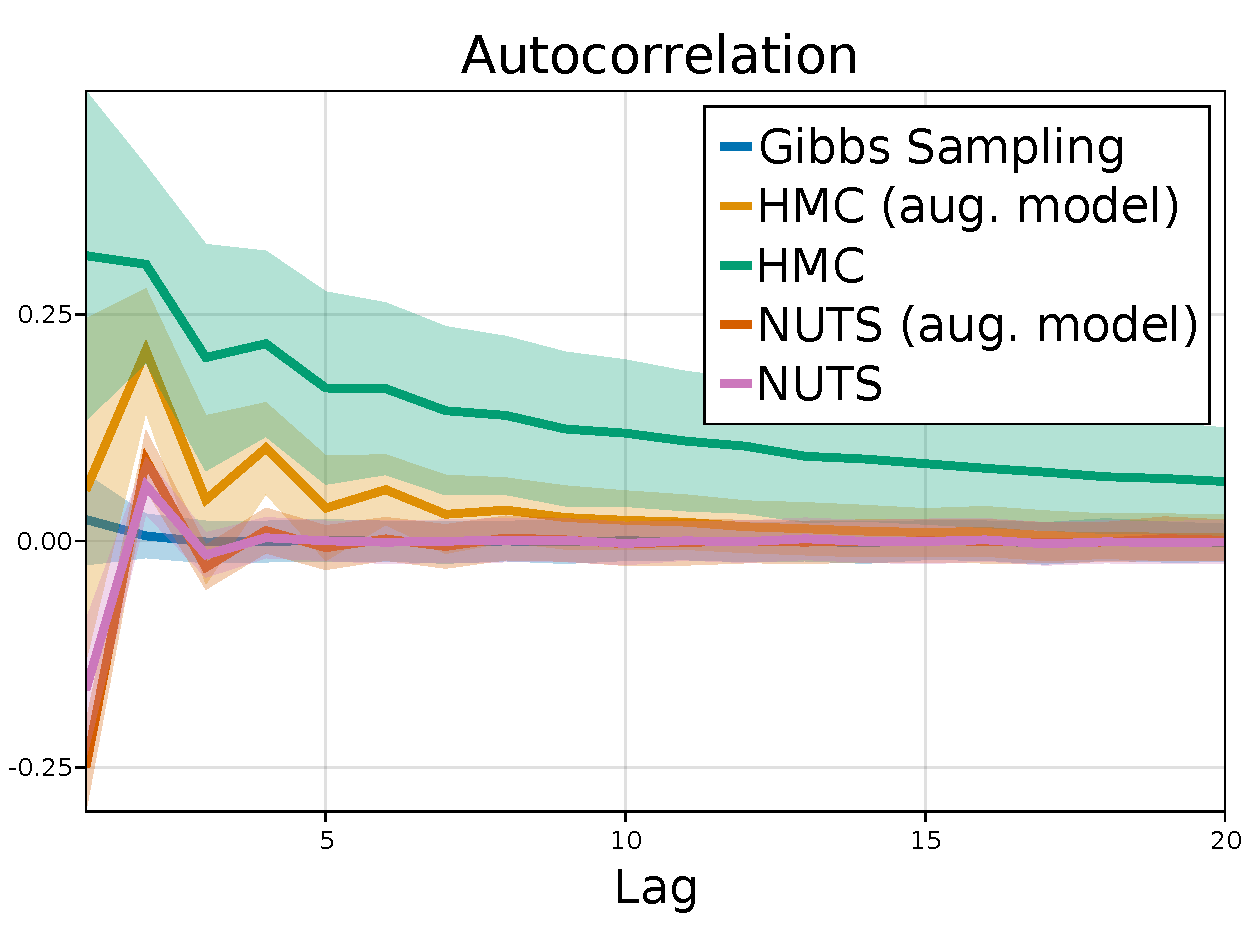
\includegraphics[width=0.5\textwidth]{./chapters/8_discussions/figures/autocorrelation.pdf}
    \caption{Auto-correlation function of the Gibbs sampler, \ac{HMC} and \ac{NUTS} on the augmented model, and \ac{HMC} and \ac{NUTS} on the original model.
    The mean is shown with one standard-deviation over all dimensions.}
    \label{fig:hmc_vs_gibbs}
\end{figure}

\section{Improvements on the Multi-Class Classification}
\label{sec:improvemulticlass}
We recently figured out additional ways to improve the multi-class classification model and the associated inference.
We present them here in 3 different sections.

\subsection{Marginalizing out variables}
\label{sec:marg_multiclass}
In the augmentation derived in Chapter~\ref{ch:multi-class}, we add $2K + 1$ new variables per observation: $\lambda$, $\{n_i\}_{i=1}^K$ and $\{\omega_i\}_{i=1}^K$.
However, we can reduce this number to $2K$ and avoid unnecessary inner loops by marginalizing out $\lambda$.
When deriving the augmentations, one ends up with the following augmented likelihood:
\begin{align}
    p(y=k, \{n_j\}_{j=1}^K, \lambda|\{f_j\}_{j=1}^K) = \sigma(f_k) \prod_{j=1}^K \sigma(-f_j)^{n_j} \Po (n_j|\lambda),
\end{align}
where we omitted the improper prior $1_{[0,\infty)}$ on $\lambda$.
We can marginalize out $\lambda$:
\begin{align}
    \int_{0}^\infty \prod_{j=1}^K \sigma(-f_j)^{n_j} \Po (n_j|\lambda)d\lambda =& \frac{1}{\prod_{j=1}^K n_j!}\int_{0}^\infty \lambda^{\sum_{j=1}^K n_j}e^{-K\lambda}d\lambda \nonumber\\
    =& \frac{K^{-\sum_{j=1}^K n_j}}{\prod_{j=1}^K n_j!}\prod_{j=1}^K \sigma(-f_j)^{n_j} \int_{0}^\infty (K\lambda)^{\sum_{j=1}^K n_j}e^{-K\lambda}d\lambda \nonumber\\
    =& \prod_{j=1}^K\sigma(-f_j)^{n_j}\Gamma(1 + \sum_{j=1}^K n_j) \prod_{j=1}^K \left(\frac{1}{K}\right)^{n_j}\frac{1}{n_j!}. \label{eq:NM}
\end{align}

Which is proportional to a \textbf{Negative Multinomial} $\operatorname{NM}(x_0, \boldsymbol{p})$ defined by:
\begin{align*}
    \operatorname{NM}(\bx|x_0,\boldsymbol{p}) = \Gamma\left(\sum_{j=0}^K x_j\right) \frac{p_0^{x_0}}{\Gamma(x_0)}\prod_{j=1}^K \frac{p_j^{x_j}}{x_j!}   
\end{align*}
with parameters $x_0=1$, $\boldsymbol{p}=\left\{\frac{\sigma(-f_j)}{K}\right\}_{j=1}^K$, and where $p_0 = 1 - \sum_{j=1}^K p_j$.
Note that the normalization term $p_0$ is missing in Equation~\eqref{eq:NM}.
However, we do not add it, as it would render the likelihood unusable.
We keep the prior unnormalized, but this does not influence the inference, as in Chapter~\ref{ch:multi-class}, since all full conditionals are available in closed-form and normalized.

These derivations could have been avoided by noticing that the \ac{MGF} of a negative binomial distribution is given by:
\begin{align*}
    \operatorname{MGF}_{\operatorname{NM}(x_0,\boldsymbol{p})}(\boldsymbol{t}) = \left(\frac{p_0}{1-\sum_{j=1}^K p_j e^{t_j}}\right)^{x_0}.
\end{align*}


Both the Gibbs sampling and \ac{CAVI} updates based on this marginalization are described in Algorithms~\ref{alg:gibbs_multiclass} and~\ref{alg:cavi_multiclass}.


\subsection{A new model for the multi-class classification}
\label{sec:simplex}
In Chapter \ref{ch:multi-class}, two concerns can be raised.
First, the parametrization of a categorical distribution with $K$ categories requires only $K-1$ independent parameters $\boldsymbol{p}$ due to the constraint $\sum_{j=1}^K p_j = 1$.
However, in the original model, which we will call \textbf{over-parametrized}, we consider $K$ independent parameters.
Second, the augmented variable $\lambda$ has the improper prior $p(\lambda) = 1_{[0,\infty)}$, which is a proper measure but is not normalizable.
It is not an important concern since \textbf{the posterior is normalizable} despite the improper prior.
Nevertheless, one might argue that improper priors should be avoided, as it does not allow model comparison.

On a side note, the fact that augmentations with improper priors still lead to valid inference is a good indication that scale mixtures for augmentation can be extended to non-normalizable measures.

These two issues seem connected, but we do not have any proof for it.

We propose an alternative parametrization with $K-1$ latent \acp{GP}.
The likelihood stays the same but with one latent being fixed:
\begin{align}
    p(y=k|\{f_j\}_{j=1}^{K-1}) = \left\{
        \begin{array}{cc}
            \frac{\sigma(f_k)}{D + \sum_{j=1}^{K-1}\sigma(f_j)}, & \mathrm{if}\; 1 \leq k < K - 1\\
            \frac{D}{D + \sum_{j=1}^{K-1}\sigma(f_j)}, & \mathrm{if}\; k = K - 1 \\
    \end{array}
    \right.,\label{eq:simplex_multiclass}
\end{align}
where $D = \sigma(f_K) \in [0, 1]$.
We call this version of the likelihood \textbf{bijective} since the dimensionality of the simplex output is the same as the inputs.

This likelihood comes with different properties.
Unlike the softmax link, the logistic-softmax link is not translation invariant\footnote{There is no function $f(\Delta)$ such that $\sigma(x + \Delta) = f(\Delta)\sigma(x)$ for all $x$.}.
We can not freely exchange classes, and the "fixed" class has a different behavior than the rest.
For example, since we fix $D$, the probability for classes other than $K$ will be upper bounded by $\frac{1}{D + 1}$.
For example, taking $D=0.5$ ($f_K = 0$) leads to a maximum probability of $1$ for the class $K$ and $2/3$ for all other classes.
On the other hand, if $D=0$, the probability of the class $K$ will always be $0$.
The bijective likelihood can still be practical if we do not care about one of the classes.
Additionally, the scaled model presented in the next Section~\ref{sec:scale_multiclass} can also help with the imbalance between classes.

Starting from the likelihood in Equation~\ref{eq:simplex_multiclass} the first augmentation that led to an improper prior in the over-parametrized model of Chapter~\ref{ch:multi-class}:
\begin{align*}
    \frac{1}{\sum_{j=1}^{K} \sigma(f_j)} = \int_0^\infty e^{-\lambda  \sum_{j=1}^{K} \sigma(f_j)}d\lambda
\end{align*}
is replaced by the known \ac{MGF} of a Gamma distribution with the following mixture:
\begin{align*}
    \frac{1}{D + \sum_{j=1}^{K-1} \sigma(f_j)} =& \frac{1}{D + \sum_{j=1}^{K-1} \sigma(f_j)} = \frac{1}{D}\frac{1}{1+\frac{1}{D}\sum_{j=1}^{K=1}\sigma(f_j)}\\
    =& \frac{1}{D}\int_0^\infty e^{-\lambda \sum_{j=1}^{K-1} \sigma(f_j)}\Ga \left(\lambda|1, \frac{1}{D}\right)d\lambda,
\end{align*}
which is true for $D > 0$.

The next augmentations steps are the same for the bijective and over-parametrized models:
We use the \ac{MGF} of the Poisson distribution and finally the P\'olya-Gamma augmentation.
We show the whole derivations on Algorithms~\ref{alg:gibbs_multiclass} and~\ref{alg:cavi_multiclass} and show an example on Figure~\ref{fig:bijective_multiclass}.
We show 1-dimensional examples with 3 classes with and without the bijection on Figure~\ref{fig:bijective_multiclass} and~\ref{fig:multiclass}
\begin{algorithm}[H]
    \caption{Gibbs sampling updates: $\textcolor{sb1}{K}/\textcolor{sb2}{K - 1}$ latent \acp{GP} for $K$ classes}
    \begin{algorithmic}
    \State \textbf{input:} $\boldsymbol{F} = \{\boldf_k\}_{k=1}^K$, $p(\boldsymbol{F}) = \prod_{k=1}^{\textcolor{sb1}{K}/\textcolor{sb2}{K - 1}} p(\boldf_k|\bmu_0, K_{\bX})$, $Y=\{\boldy^i\}_{i=1}^N$ (one-hot encoded)
    \For{$t$ in 1: \# samples}
        \State Draw $\boldsymbol{n}^i \sim p(\boldsymbol{n}^i|\boldsymbol{F}) = \mathrm{NM}(1, \boldsymbol{p}^i)$ where 
        $p_k^i = \textcolor{sb1}{\frac{\sigma(-f_k^i)}{K}}/\textcolor{sb2}{\frac{\sigma(-f_k^i)}{D + K - 1}}$
        \State Draw $\omega_k^i \sim p(\omega_k^i|f_k^i, n_k^i, y_k^i) = \PG(y_k^i + n^i_k, |f_k^i|)$
        \State Draw $\boldf_k \sim p(\boldf_k|\bomega_k,\boldsymbol{n}_k, \boldsymbol{Y}) = \mathcal{N}(\boldm_k, \boldsymbol{S}_k)$
        \State where $\boldsymbol{S}_k = \left(K_{\bX}^{-1} + \diag(\bomega_k)\right)^{-1}$ and $\boldm_k = \boldsymbol{S}_k\left(K^{-1}_{\bX}\bmu_0 + \frac{\boldy_k - \boldsymbol{n}_k}{2}\right)$
    \EndFor
    \end{algorithmic}
    \label{alg:gibbs_multiclass}
\end{algorithm}

\begin{algorithm}[H]
    \caption{\ac{CAVI} updates: $\textcolor{sb1}{K}/\textcolor{sb2}{K - 1}$ latent \acp{GP} for $K$ classes}
    \begin{algorithmic}
    \State \textbf{input:} $q(\boldsymbol{F}) = \prod_{k=1}^{\textcolor{sb1}{K}/\textcolor{sb2}{K - 1}} q(\boldf_k|\bmu_k, \bSigma_k)$, $p(\boldsymbol{F} = \prod_{k=1}^{\textcolor{sb1}{K}/\textcolor{sb2}{K - 1}} p(\boldf_k|\bmu_0, K)$, $Y=\{\boldy^i\}_{i=1}^N$ (one-hot encoded)
    \While{convergence criteria is not met}
        \State $c^i_k = \sqrt{(\mu^i_k)^2 + \Sigma_k^{ii}}$
        \State $p^i_k = \textcolor{sb1}{\frac{\widetilde{\sigma}(q(f_k^i))}{K}}/\textcolor{sb2}{\frac{\widetilde{\sigma}(q(f_k^i))}{D + K - 1}}$
        \State $\bgamma^i = \expec{q(\boldsymbol{n}^i)}{\boldsymbol{n}^i} = \frac{\boldsymbol{p}^i}{1 - \sum_{i=1}^K p^i_k}$
        \State $\theta_k^i = \expec{q(\omega_k^i)}{\omega_k^i} = \frac{y_k^i + \gamma_k^i}{2c_k^i}\tanh\left(\frac{c_k^i}{2}\right)$
        \State $\bSigma_k = \left(K_{\bX}^{-1} + \diag(\boldsymbol{\theta}_k)\right)^{-1}$
        \State $\bmu_k = \bSigma_k\left(K_{\bX}^{-1}\bmu_0 + \frac{\boldy_k - \bgamma_k}{2}\right)$
    \EndWhile
    \end{algorithmic}
    where $q(\boldsymbol{N}, \bOmega) = \prod_{i=1}^N \PG(\bomega^i|\boldy^i + \boldsymbol{n}^i, \boldsymbol{c}^i)\mathrm{NM}(\boldsymbol{n}^i|1, \boldsymbol{p}^i)$ and $\widetilde{\sigma}(q(f_k^i)) = \frac{e^{-\mu_k^i/2}}{\sqrt{(\mu_k^i)^2 + \Sigma^{ii}_k} / 2}$ is an approximation to the $\sigma(-f^i_k)$.
    \label{alg:cavi_multiclass}
\end{algorithm}

\begin{figure}[H]
    \centering
    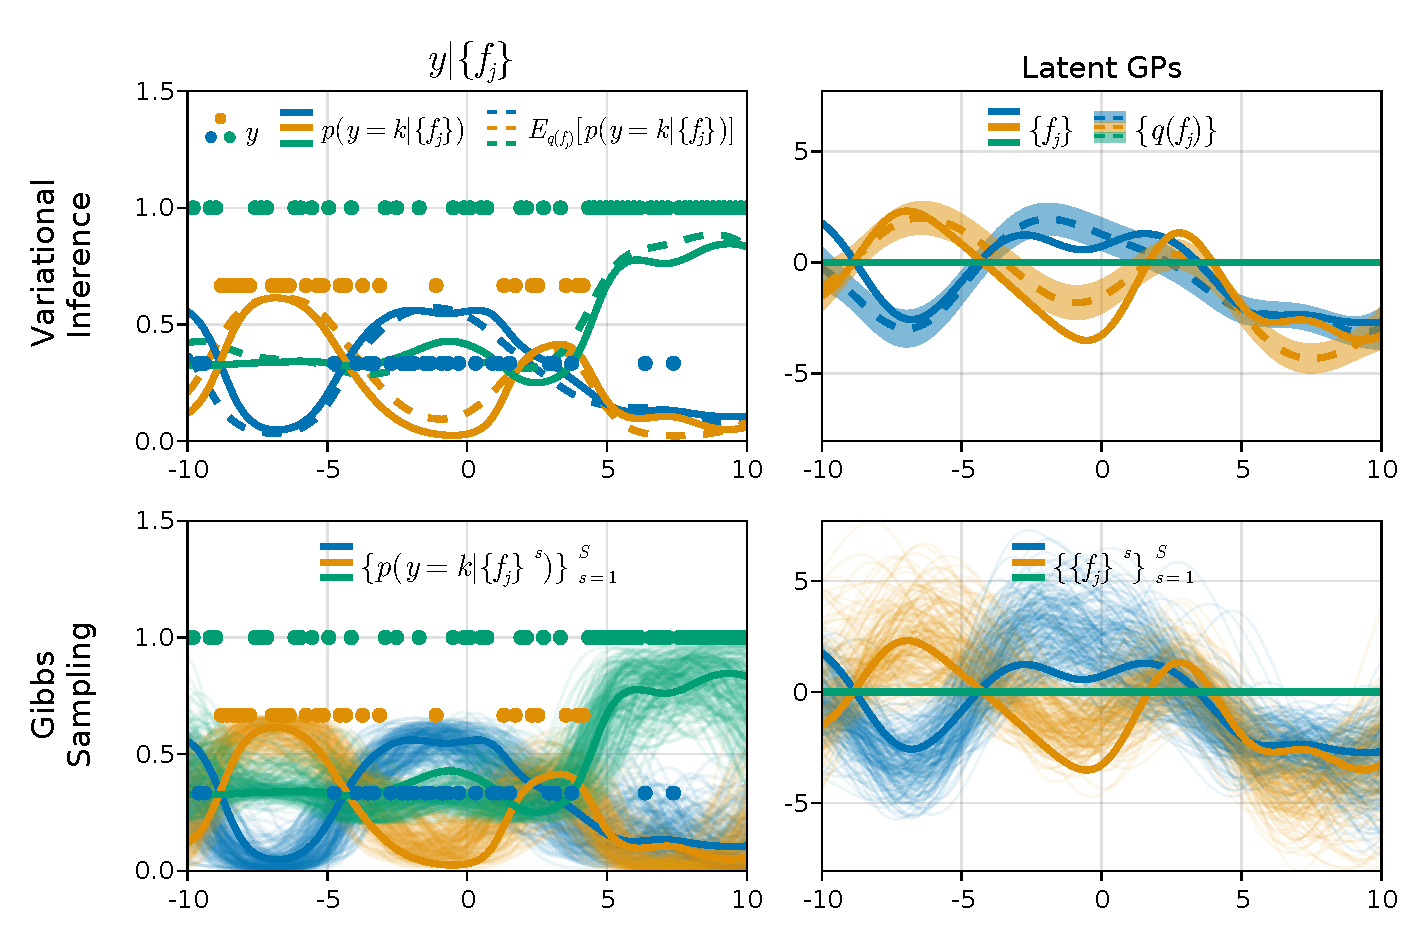
\includegraphics[width=\textwidth]{./chapters/8_discussions/figures/categorical_bijective.pdf}
    \caption{Illustration of Algorithms~\ref{alg:gibbs_multiclass} and~\ref{alg:cavi_multiclass} with the bijective link introduced in Section~\ref{sec:simplex} and the marginalization of Section~\ref{sec:marg_multiclass}.
    Each color represents a class, and we compare the true process to the inferred one for both Gibbs sampling and variational inference.
    The solid lines represent the true probabilities and latent \acp{GP}.
    The plots on top show the variational inference results, with the expected predictive probability on the left and the variational posterior on the right.
    The plots at the bottom show the probabilities and latent \acp{GP} obtained via Gibbs sampling.}
    \label{fig:bijective_multiclass}
\end{figure}
\begin{figure}[H]
    \centering
    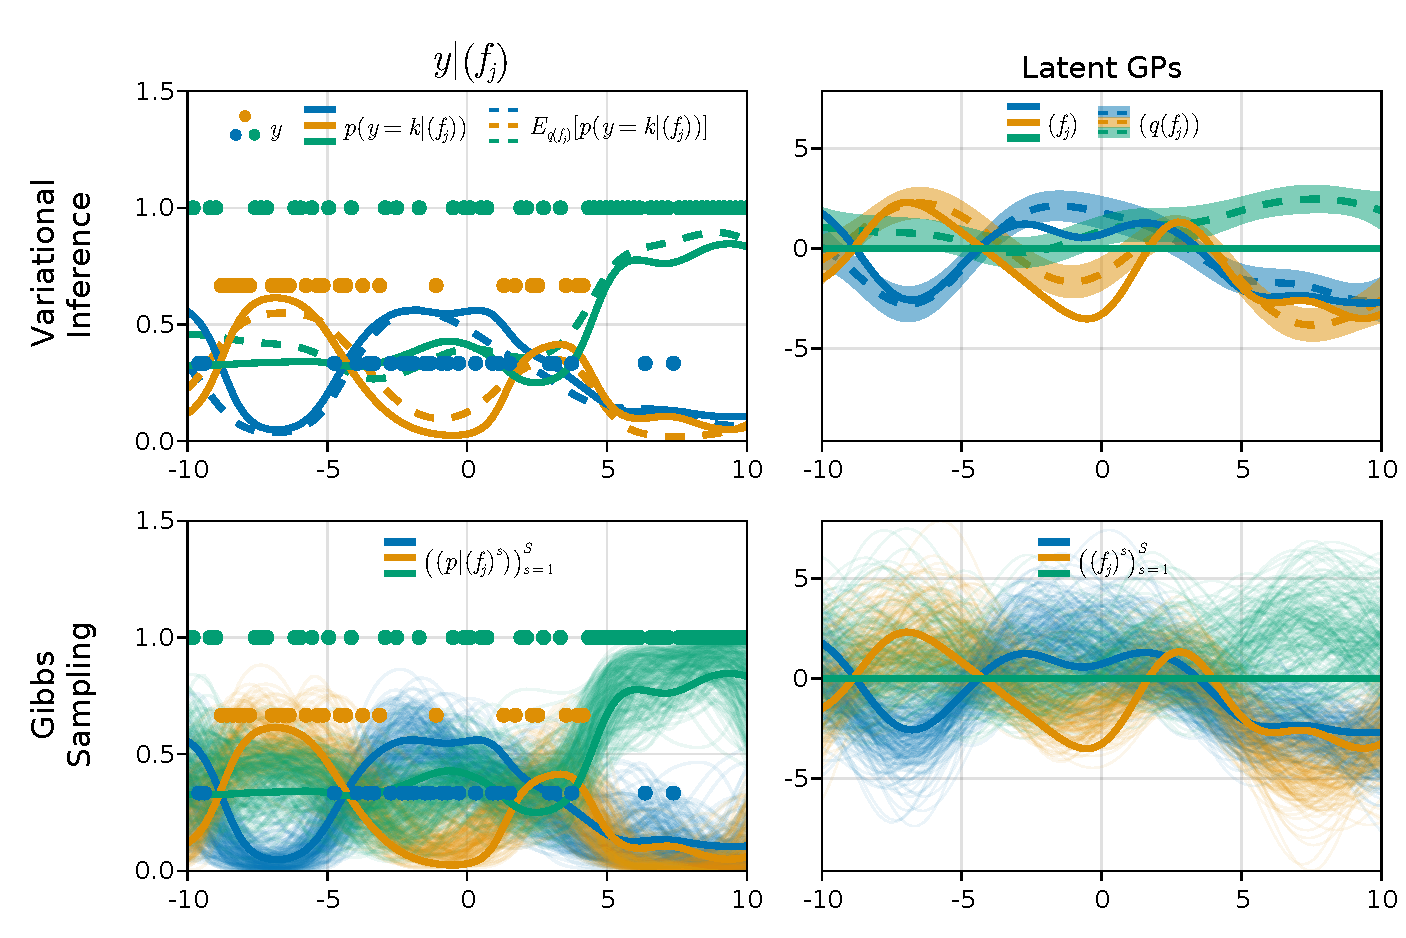
\includegraphics[width=\textwidth]{./chapters/8_discussions/figures/categorical_nonbijective.pdf}
    \caption{Illustration of Algorithms~\ref{alg:gibbs_multiclass} and~\ref{alg:cavi_multiclass} with the overparametrized link with the marginalization of Section~\ref{sec:marg_multiclass}.
    Each color represents a class, and we compare the true process to the inferred one for both Gibbs sampling and variational inference.
    The solid lines represent the true probabilities and latent \acp{GP}.
    The plots on top show the variational inference results, with the expected predictive probability on the left and the variational posterior on the right.
    The plots at the bottom show the probabilities and latent \acp{GP} obtained via Gibbs sampling.}
    \label{fig:multiclass}
\end{figure}

Both the bijective and over-parametrized links fit correctly this one-dimensional example.
The over-parametrized link in Figure~\ref{fig:multiclass} do not approximate correctly the fixed latent $f_K=0$ but still returns good predictive distributions.

When repeatedly running these examples, we observe that the predictive probabilities for the bijective link are consistently more accurate, but the predictive log-likelihood for the correct class is higher on the over-parametrized link.
To confirm this trend, we would need further experiments on real datasets and with a higher number of classes. 

\subsection{Scaling the logistic-softmax link}
\label{sec:scale_multiclass}
The logistic-softmax link has issues with the predictive probabilities, in particular with many classes.
Because of the boundedness of the logistic function, the logistic-softmax link needs large values of $f_i$ to reach prediction probabilities close to $1$.
Even when the model should be very confident about a prediction and the latent \acp{GP} are correctly inferred, the predictive probability for the correct class will be around $(1-\epsilon) / ((K - 1) \epsilon +  1 - \epsilon)$ where $\epsilon$ is the minimum value taken by $\sigma(f)$.
With a \ac{GP} prior centered at 0 and a reasonable kernel variance, $f$ can not take large values.
For example, taking 10 classes, if we assume $f_y=4$ for the correct class and $-4$ for the others, $\epsilon \approx 0.018$, which gives a probability of $0.858$ with the logistic-softmax link against $0.996$ for the softmax link.

This can be solved by using a scaled logistic function.
We add $K$ hyperparameters $\btheta=\{\theta_{i}\}_{i=1}^K$ such that the likelihood becomes
\begin{align*}
    p(y=k|\{f_j\}_{j=1}^K,\btheta) = \frac{\theta_k \sigma(f_k)}{\sum_{j=1}^K \theta_j \sigma(f_j)}.
\end{align*}
The $\btheta$ parameters can be optimized using the \ac{ELBO} with the other hyperparameters.
These can also provide information about each class, a high $\theta_j$ meaning that the $j$-th class has zones of very high confidence.
With the likelihood augmented with the variable $\lambda$, the collapsed-conditional and the maximum-likelihood optimum of $\btheta$ is available in closed-form.
The maximum-likelihood optimizer is given by:
\begin{align*}
    \theta^*_k = \frac{\sum_{i=1}^N \delta(y^i, k)}{\sum_{i=1}^N \expec{q(\lambda^n)}{\lambda^n}(1 - \widetilde{\sigma}(q(f_k^i)))},
\end{align*}
where $\delta(x,y)$ is the Kronecker delta function, equal to 1 if $x=y$ and 0 otherwise and where $\widetilde{\sigma}(q(f_k^i))$ is defined as in Algorithm~\ref{alg:cavi_multiclass}.
We used the model definition where $\lambda$ is not marginalized out.

By putting a prior $\mathrm{Ga}(\theta_k|\alpha,\beta)$, the collapsed conditional of each $\theta_k$ is given by:
\begin{align*}
    p(\theta_k|\boldf_k, \boldsymbol{\lambda}) = \mathrm{Ga}(\theta_k|\alpha + \sum_{i=1}^N\delta(y^i, k), \beta + \sum_{i=1}^N\lambda^i\sigma(f_k^i))
\end{align*}

A Julia implementation as well as detailed derivations can be found in the \href{https://github.com/JuliaGaussianProcesses/AugmentedGPLikelihoods.jl}{\texttt{AugmentedGPLikelihoods.jl}} package \cite{theo_galy_fajou_2022_6347022}.

\section{Sampling from a sparse augmented model}
\label{sec:sample_sparse}
Another work in progress regards the sampling of sparse \acp{GP} models.
Sampling from the augmented model proves to be very effective (see Chapter~\ref{ch:general}) while still producing samples from the posterior $p(\boldf|\boldy)$ of the original model.
Unfortunately, this property does not transfer when using sparse \acp{GP} (for a reminder on sparse \acp{GP}, see Section~\ref{sec:sparsegps}) and the scalability is limited.
Simply adding inducing points locations $Z$ with realizations $\boldu = f(Z)$ leads to a Gibbs sampling algorithm with a computational complexity of $\mathcal{O}((N+M)^3)$ per step and does not help with scalability.
To solve this problem, we propose to mix the Gibbs sampling approach we presented in Chapter~\ref{ch:general} with variational inference.

We build on the work of \citet{hensmanMCMCVariationallySparse2015}. 
They make the Titsias' assumption \cite{Titsias2009}, i.e. setting the variational distribution as $q(\boldu,\boldf) = q(\boldu)p(\boldf|\boldu)$.
Since they also assume a fully factorizable likelihood $p(\boldy|\boldf) = \prod_{i} p(y_i|f_i)$, only marginals $q(f_i)$ are required and the computational complexity of the bound decreases to $\mathcal{O}(NM^2 + M^3)$.  
\citet{hensmanMCMCVariationallySparse2015} show the optimal variational distribution of the inducing variables $\boldu$ minimizing $\KL{q(\boldu, \boldf)}{p(\boldu)p(\boldf|\boldu)p(\boldy|\boldf)}$ for a factorizable likelihood $p(\boldy|\boldf)=\prod_i p(y_i|f_i)$ is given by:
\begin{align}
    \log q^*(\boldu) = \sum_{i}\expec{p(f_i|\boldu)}{\log p(y_i|f_i)} + \log p(\boldu) + C,\label{eq:obj_hensman}
\end{align}
where $C$ is an intractable constant.
$q^*(\boldu)$ does not have a specific form in the general case, but we can sample from it by using \ac{HMC} and evaluating the integrals $\expec{p(f_i|\boldu)}{\log p(y_i|f_i)}$ numerically\footnote{With quadrature for low-dimensions} as in \cite{hensmanMCMCVariationallySparse2015}.

We propose instead to derive a variational Gibbs sampling algorithm to draw samples from the variational distribution minimizing the Renyi divergence \cite{van2014renyi} defined as
\begin{align}
    D_\alpha(p,q) = \frac{1}{\alpha(\alpha - 1)}\log\int \alpha p(x) + (1-\alpha)q(x) - p^\alpha(x)q^{1-\alpha}(x)dx,\quad \alpha \in \mathbb{R}^+.\label{eq:renyi}
\end{align}
The Renyi divergence converges to the forward KL divergence: $\KL{p}{q}$ for $\alpha=1$ and the reverse KL divergence: $\KL{q}{p}$ for $\alpha=0$ \cite{van2014renyi}.
We define our variational distribution as $q(\boldu,\boldf,\bOmega) = q(\boldu,\bOmega)\prod_i p(f_i|\boldu)$, and aim at minimizing $D_\alpha(p(\boldu,\boldf,\bOmega|\boldy),q(\boldu,\boldf,\bOmega))$.
Note that we do not assume any independence between $\boldu$ and $\bOmega$, only that every $f_i$ is conditionally independent given $\boldu$.
There is no parametric closed-form for the optimal distribution $q^*(\boldu,\bOmega)$ minimizing the divergence in Equation~\eqref{eq:renyi}, hence we take the approach of \citet{hensmanMCMCVariationallySparse2015} and sample from it instead.
We draw $\boldu$, $\boldf$ and $\bOmega$ with a blocked Gibbs sampler, by sampling from the optimal variational distribution minimizing the conditional Renyi divergences:
\begin{align}
    \bOmega^i \sim q^*(\bOmega) =& \arg_q \min D_\alpha\left(p(\bOmega|\boldu^{i-1},\boldf^{i-1},\boldy),q(\bOmega)\right)\label{eq:var_omega}\\
    \boldu^i, \boldf^i \sim q^*(\boldu,\boldf) =& \arg_q \min D_\alpha\left(p(\boldu,\boldf|\bOmega^i,\boldy),q(\boldu,\boldf)\right)\nonumber\\
    =& \arg_q \min D_\alpha\left(p(\boldu)p(\boldf|\boldu)p(\boldf|\bOmega^i,\boldy),q(\boldu)\prod_i p(f_i|\boldu)\right).\label{eq:var_uf}
\end{align}
For all $\alpha$, the minimizer for $q^*(\bOmega)$ is $p(\bOmega|\boldu^{i-1},\boldf^{i-1},\boldy)$, setting the conditional divergence to 0.
With the approach from Chapter~\ref{ch:general}, we know $p(\bOmega|\boldu,\boldf,\boldy)$ (which can be simplified to $p(\bOmega|\boldf,\boldy)$) in closed-form and can sample from it with linear complexity with respect to the number of data points.

\citet{buiUnifyingFrameworkGaussian2017} solved the optimization problem of Equation~\eqref{eq:var_uf} for Gaussian likelihoods, with the \textbf{Power-EP} algorithm.
Since $p(\boldf|\bOmega,\boldy)$ is conjugate in $\boldf$, the optimal $q^*(\boldu)$ is a multivariate normal distribution with the mean and variance known in closed-form for all $\alpha \in \mathbb{R}^+$.
Each sampling step for $\boldu$ and $\boldf$ only has complexity $\mathcal{O}(M^3 + M^2N)$.
Like in the Power-EP setting, $\alpha=0$ corresponds to solving the variational approach of \citet{Titsias2009}, while $\alpha=1$ corresponds to solve the Fully Independent Training Conditional (FITC) approach of \citet{snelsonSparseGaussianProcesses2009}, as shown in \citet{buiUnifyingFrameworkGaussian2017}.

The only parameters left are the hyperparameters $\btheta$, omitted in the previous equations, that can represent a real challenge.
For $\alpha=0$, we could sample from $q^*(\btheta)$ with the \ac{HMC} algorithm in a separate Gibbs sampling step.
For other $\alpha$, we could optimize $q(\btheta)$ with variational inference methods \cite{li2016renyi, hernandez2016black}, and hot-start with the previous distribution.
The complete variational Gibbs sampler is described in Algorithm~\ref{alg:sparsegp}.

\begin{algorithm}[H]
    \caption{Variational Gibbs Sampler for Sparse \acp{GP}}
    \begin{algorithmic}
        \State \textbf{input:} $\boldy$, $\boldu^0 \sim p(u)$, $\boldf^0 \sim p(\boldf|\boldu^0)$, $\btheta^0 \sim p(\btheta)$
    \For{$t$ in 1: \# samples}
        \State Draw $\bOmega^i \sim p(\bOmega|\boldf^{i-1},\btheta^{i-1}\boldy)$ \textit{(in closed form)}
        \State Draw $\boldu^i,\boldf^i \sim q^*(\boldu,\boldf) = \arg_q \min D_\alpha\left(p(\boldu,\boldf|\bOmega^i,\btheta^{i-1},\boldy),q(\boldu,\boldf)\right)$ (\textit{in closed form})
        \State Draw $\btheta^i \sim q^*(\btheta^i) = \arg \min D_\alpha\left(p(\btheta|\boldu^i, \boldf^i, \bOmega^i, \boldy), q(\btheta)\right)$ (\textit{\ac{HMC} or optimization})
    \EndFor
    \end{algorithmic}
    \label{alg:sparsegp}
\end{algorithm}


Our approach completely gets rid of expectation computations for $\boldu$.
It opens up more possibilities over more complex likelihoods like the multi-class or heteroscedastic ones where computing expectations numerically, like in Equation~\eqref{eq:obj_hensman}, is a limitation.
For medium-sized datasets, this outperforms the \ac{CAVI} algorithm as it has the same convergence speed but does not suffer from the mean-field assumption on the variational parameters.
We show preliminary results on Figure~\ref{fig:magictelescope} for a binary classification problem on the Magic Telescope dataset (10 dimensions, 19020 data points) \cite{bock2004methods}.
The experiment is run with a 10-fold cross-validation, we use $M=50$ inducing points selected via the k-means++ algorithm \cite{arthur2007k}, and we keep the hyperparameters fixed.
We compare our approach (\textbf{VI-Gibbs}) with $\alpha=0$ against the \ac{HMC}\footnote{HMC is run with a fixed step-size of 0.1 and with 10 leapfrog steps.} variational sampling method of \citet{hensmanMCMCVariationallySparse2015} mentioned earlier (\textbf{VI-HMC}), a standard \ac{VI} method optimized with an L-BFGS optimizer (\textbf{Std. VI}) and the augmented \ac{VI} approach from Chapter~\ref{ch:classification} with \ac{CAVI} updates (\textbf{Aug. VI}).
We show the classification error and test negative log-likelihood over time on Figure~\ref{fig:magictelescope}.

\begin{figure}[H]
    \centering
    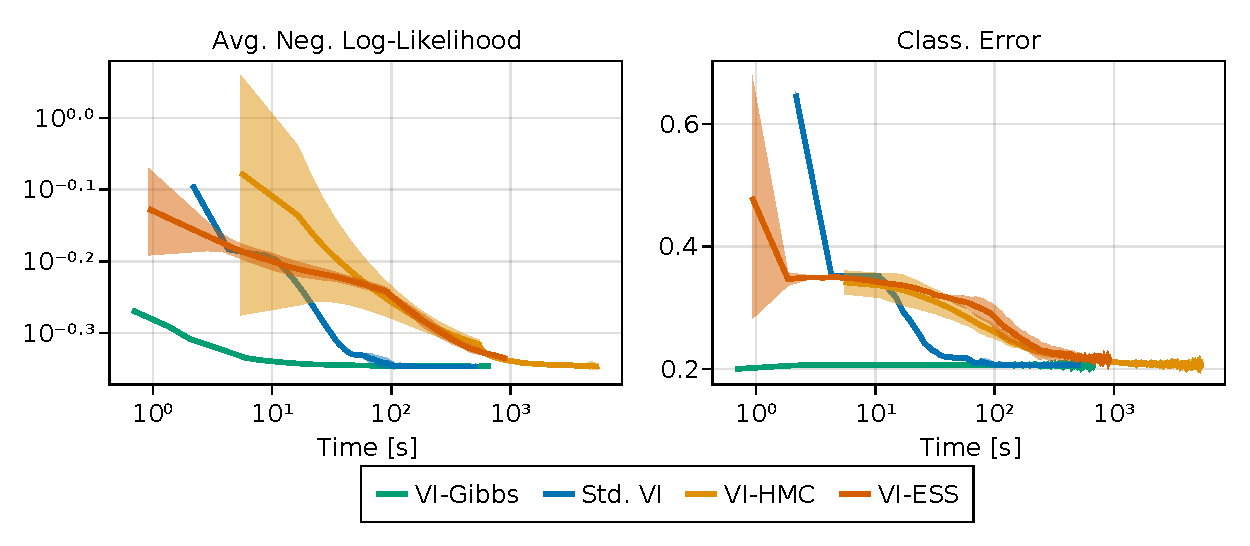
\includegraphics[width=\textwidth]{./chapters/8_discussions/figures/magictelescope.pdf}
    \caption{Negative test log-likelihood and classification test error over time on the Magic Telescope dataset.
    The mean with one standard deviation over 10 runs is shown for each algorithm.
    }
    \label{fig:magictelescope}
\end{figure}

These are first results, and there is still work on optimizing the implementation, but some first impressions can already be drawn.
In terms of iterations, VI-Gibbs is just as fast as the \ac{CAVI} updates but seem to have a slightly better optima.
It also completely outperforms methods applied on the original model.

These preliminary graphs look very promising, but adding hyperparameter sampling might slow down the process.
We also need to compare results with different likelihoods and different $\alpha$s.


% \begin{figure}[H]
%     \centering
%     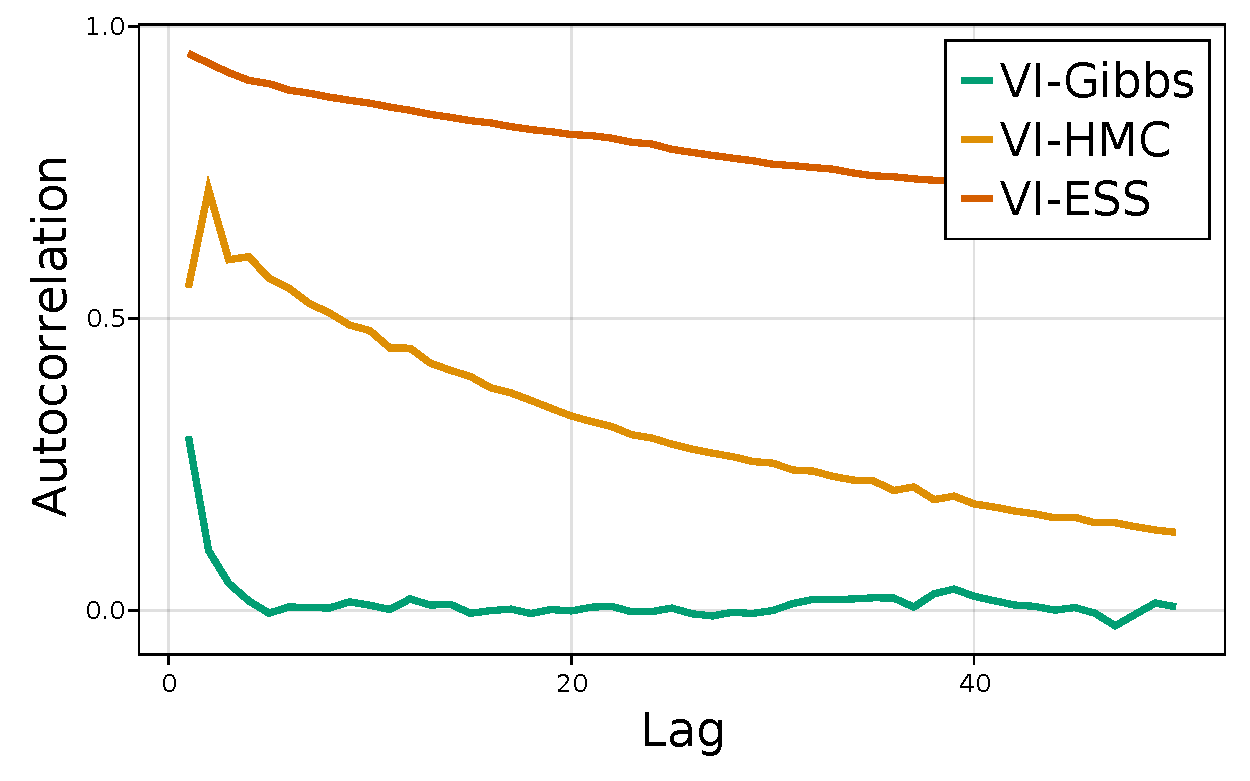
\includegraphics[width=0.5\textwidth]{./chapters/8_discussions/figures/magictelescope_autocor.pdf}
%     \caption{Intra-chain correlation against the lag for the sampling approaches.}
%     \label{fig:magictelescope_autocor}
% \end{figure}

\section{Limitations}
\label{sec:limits}
Unfortunately, augmentations are not a silver bullet for approximate Bayesian inference.
\paragraph[]{Augmentable functions}\mbox{}\\
The largest issue is naturally the limited domain of application. 
Only a constrained set of functions can be augmented.
The idea of generalization using \ac{MGF} as mentioned in Section~\ref{sec:further} is promising but limited nonetheless.
When they exist, the identification of augmentable functions in a given model can be tedious and may require lengthy derivations.
We often need to rearrange terms and use mathematical identities before applying procedures like the ones described in this thesis.
It is accessible to someone with expertise, but automatizing this derivation process is complicated.
Current progress in symbolic programming could eventually help in this direction.
We could automate this process by having a lookup table of augmentable functions and manipulating terms symbolically.

\paragraph[]{Mean-field approximation in \ac{VI}}\mbox\\
Another issue is the variational distribution $q(\boldf, \bOmega)$ (or $q(\boldu, \bOmega)$) approximating the posterior $p(\boldf, \bOmega|\boldy)$ of the augmented model is not as accurate as the variational distribution $q(\boldf)$ (or $q(\boldu)$) approximating the posterior $p(\boldf|\boldy)$ of the original model (see Section~\ref{sec:cavi}).
Although the original model can be recovered from the augmented model by marginalizing out the augmented variables $\bOmega$, the \ac{MF} approximation loses information (correlation between $\bOmega$ and $\boldf$) and breaks this link.
Marginalizing out $\bOmega$ in $q^*(\boldf, \bOmega)$ will not return the optimal $q^*(\boldf)$ trained on the original model.
Interestingly, the bound difference comes exclusively from the mean-field assumption between $q(\boldf)$ and $q(\bOmega)$.
We can even identify these bound differences via the interpretation of \citet{jaakkolaVariationalApproachBayesian1997} as missing terms from a Taylor series, as shown in Chapter~\ref{ch:classification}.
When analyzing the quality of the predictive distributions, the variational distribution trained on the augmented model proves to be almost as good as the variational distribution trained on the original model.
The difference of bounds mentioned earlier is often not significant at convergence but will create a difference nonetheless.
These empirical results give us an indication that $\boldf$ and $\bOmega$ are naturally strongly decorrelated, which would explain why the Gibbs sampling and \ac{CAVI} updates are so efficient.
% The work of \citet{gorinovaAutomaticReparameterisationProbabilistic2020} mentioned in the introduction aims at finding a perfect balance between two parametrizations by ensuring that the posterior is as close as possible to an isotropic multivariate Gaussian with independent dimensions. \mycom{unfinished}




% ---------------------------------------------------------------------------
% ----------------------- end of thesis sub-document ------------------------
% ---------------------------------------------------------------------------
